\chapter{Lazy Load}

Fowler fornisce quattro implementazioni per questo pattern.

\section{Lazy Inizialization}

\begin{center}
    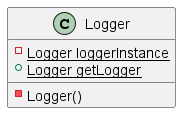
\includegraphics[width=6cm]{images/lazy-load/LoggerUML.png}
    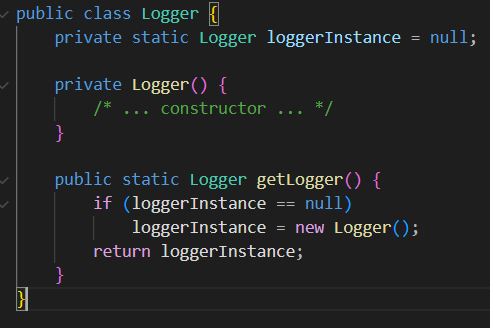
\includegraphics[width=12cm]{images/lazy-load/Logger.png}
\end{center}

In questa implementazione si controlla la disponibilita' del dato ed eventualmente si istanzia. Quindi viene ritornato.

\section{Virtual Proxy}

\begin{center}
    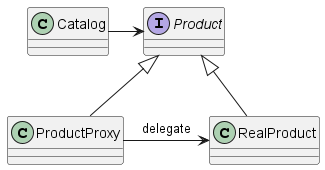
\includegraphics[width=12cm]{images/lazy-load/VirtualProxy.png}
\end{center}

Si crea una astrazione con una interfaccia e un intermediario che delega al RealProduct gli obiettivi di Product e si occupa soltanto di fornire all'occorrenza i servizi del RealProduct al Catalog.

\section{Value Holder}

\begin{center}
    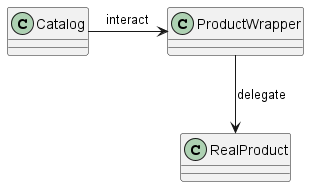
\includegraphics[width=12cm]{images/lazy-load/ValueHolder.png}
\end{center}

Si usa un ProductWrapper che assume tutte le responsabilita' che aveva il ProductProxy
La differenza con il Virtual Proxy e' che in questo caso il Catalog e' cosciente di stare interagendo con il ProductWrapper.

\section{Ghost}

\begin{center}
    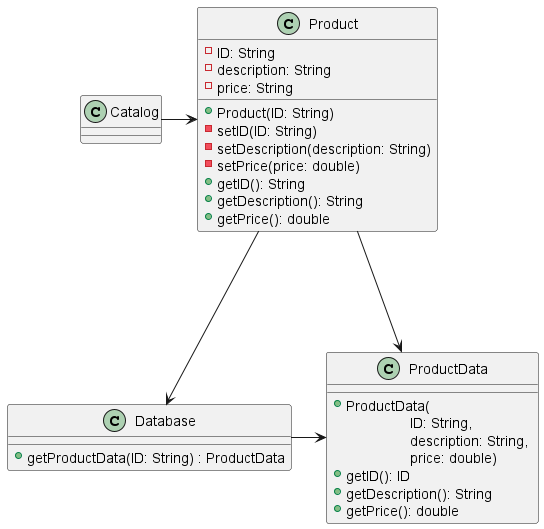
\includegraphics[width=12cm]{images/lazy-load/ProductClass.png}
    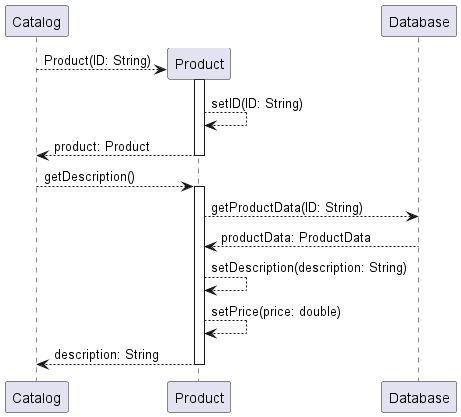
\includegraphics[width=12cm]{images/lazy-load/ProductSD.png}
\end{center}

Il Ghost qui' e' la classe Product, la quale e' un oggetto che quando viene instanziato contiene solo parte delle sue informazioni (ID), ma quando richiesto carica il resto delle informazioni.
Si noti che la classe ProductData e' immutabile, ed utilizzata solo per pattare informazioni tra il Database e il Product.
